\section{Background}
\label{sec:background}
For the background of this project, it is necessary to consider literature related to the following:
\begin{mylist}
  \item Existing computer vision systems for component identification
  \item Real-time computer vision architectures
  \item Mechanical design of existing sorting machines
\end{mylist}
Research into these topics will inform the decisions made in the design of the project and its various systems.

\begin{figure*}[t]
  \begin{minipage}[t]{0.49\textwidth}
    \centering
    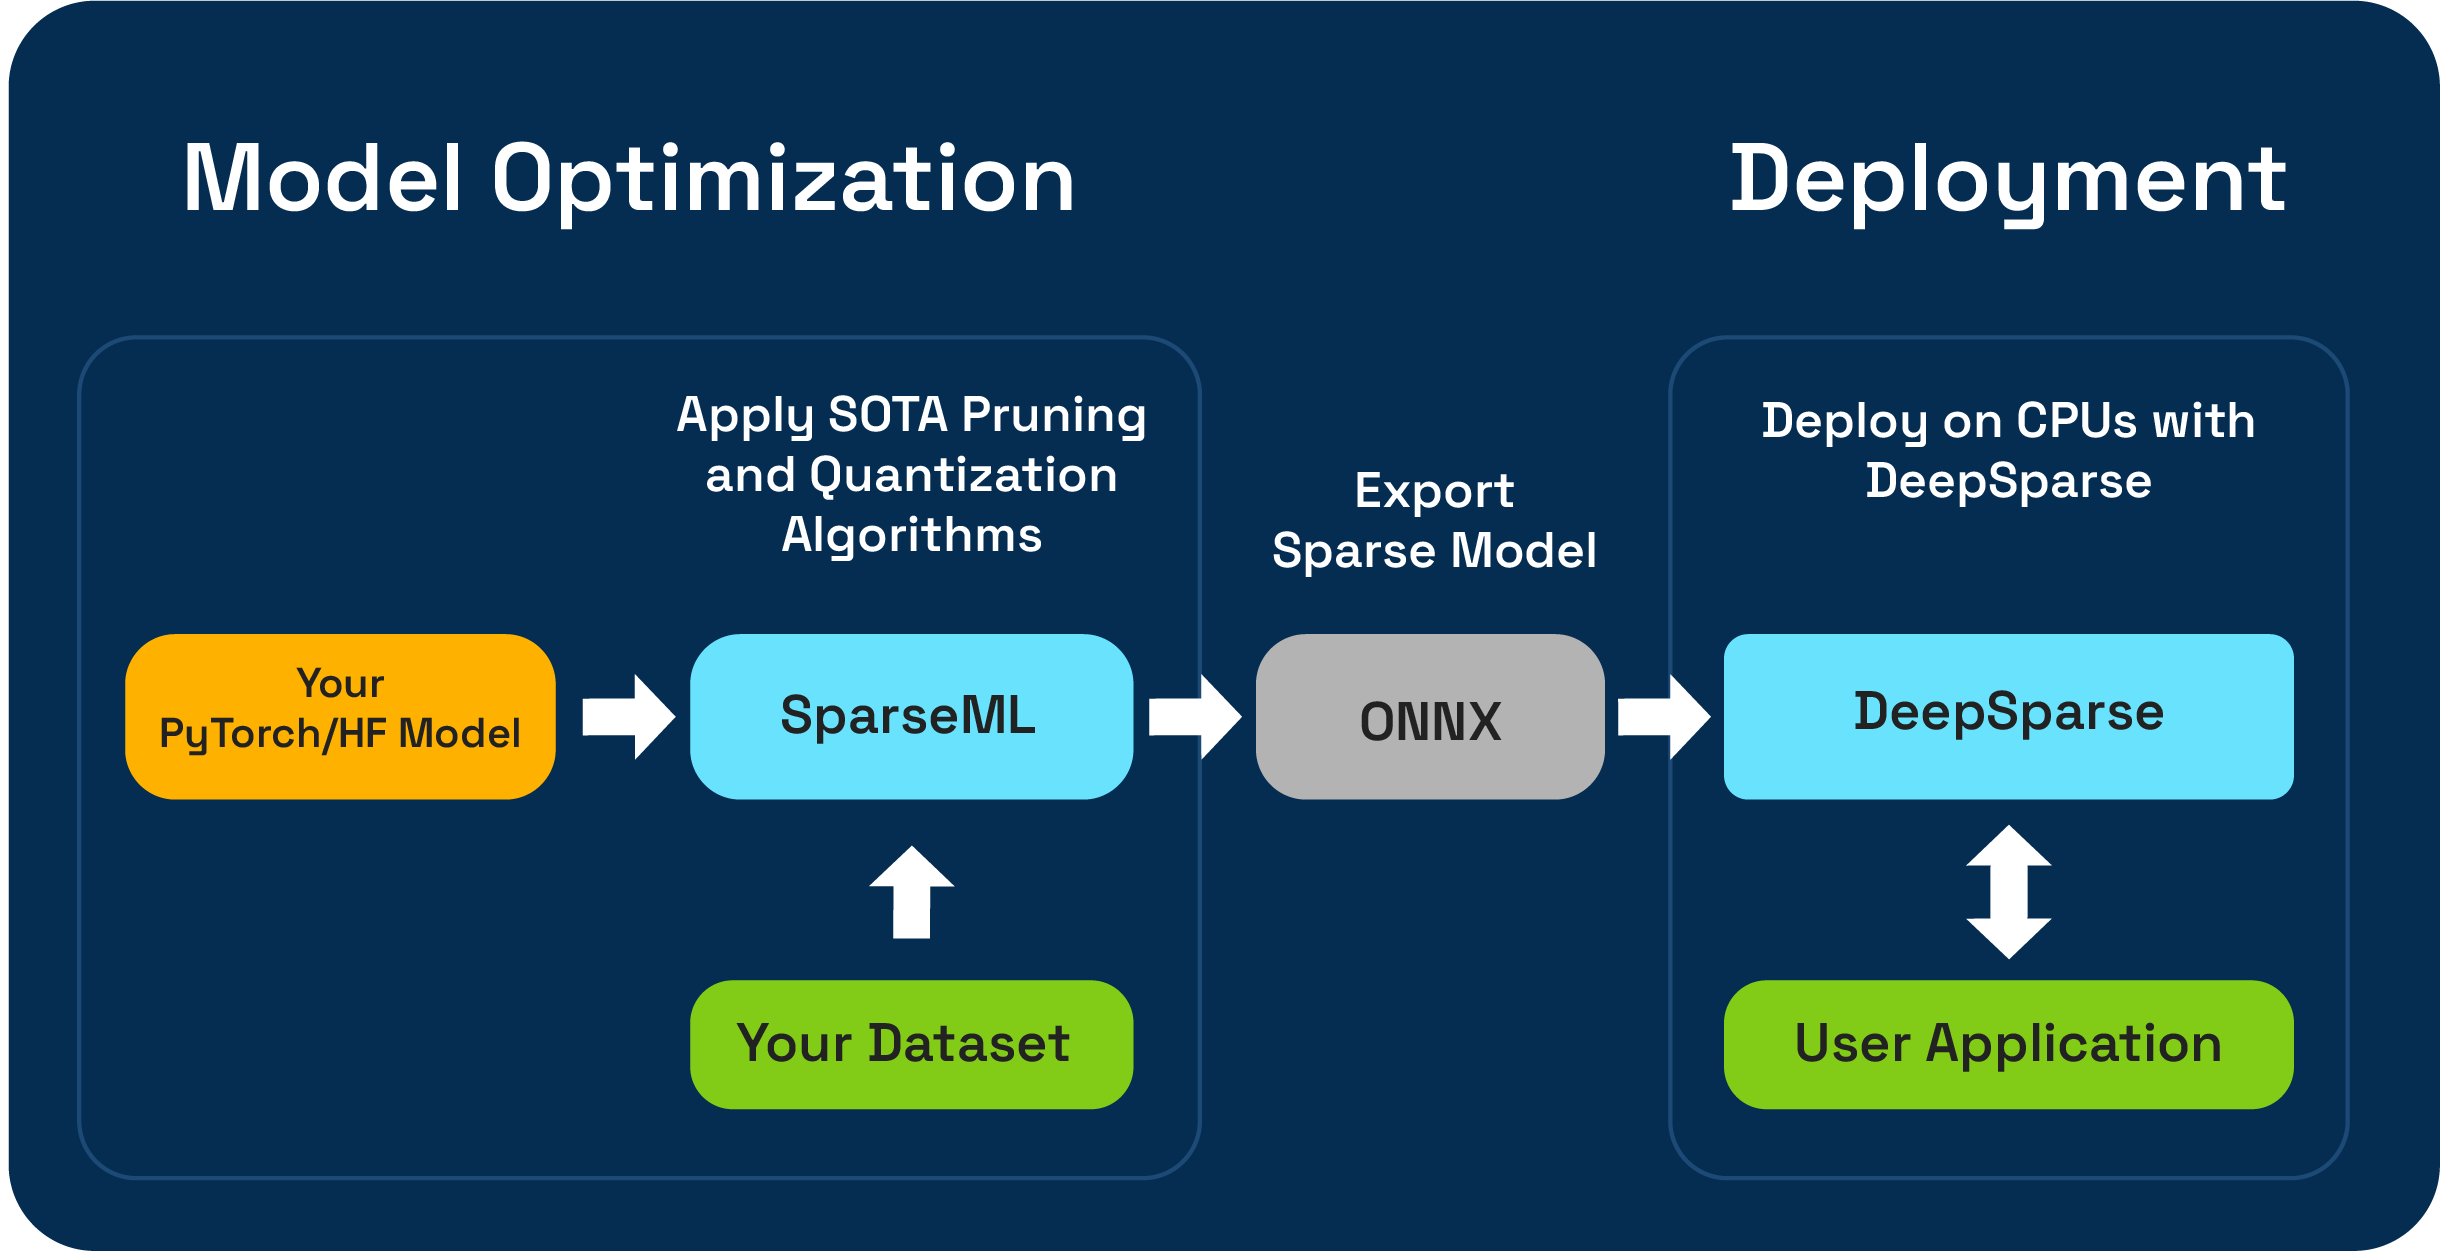
\includegraphics[width=\textwidth,height=5cm]{imgs/articles/sparseml-workflow.png}
    \caption{SparseML Pipeline \cite{sparseml}}
  \end{minipage}
  \hfill
  \begin{minipage}[t]{0.49\textwidth}
      \centering
      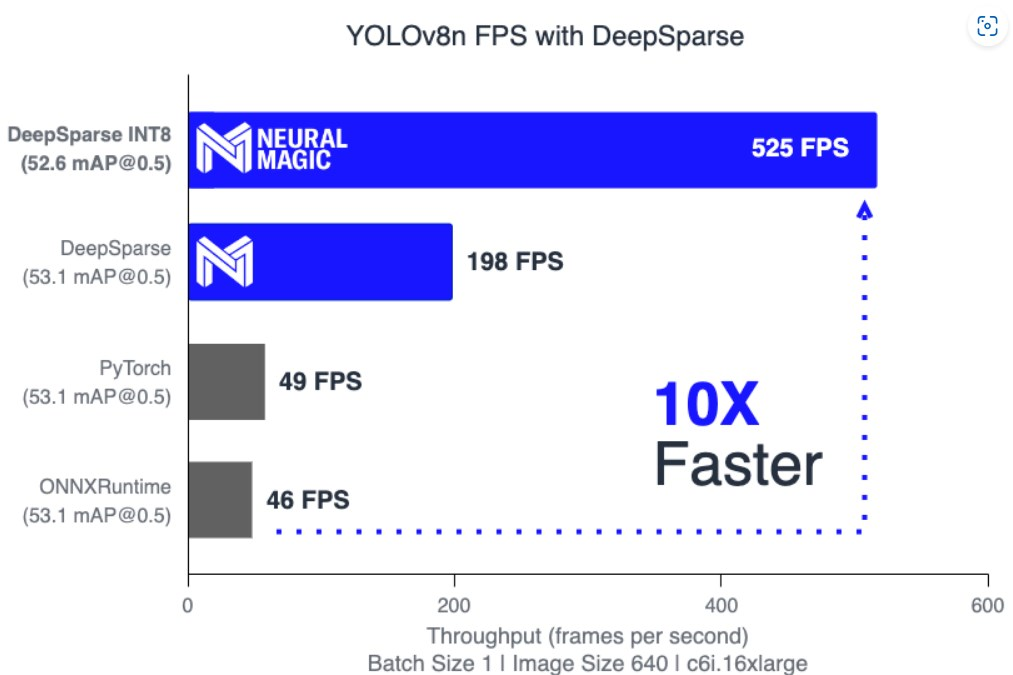
\includegraphics[width=\textwidth,height=5cm]{imgs/articles/yoloperf.jpg}
      \caption{DeepSparse Performance \cite{neuralmagic}}
      \end{minipage}
\end{figure*}

\subsection{Existing Computer Vision Systems}
A range of computer vision systems have been explored in the literature, ranging from PCA (Principle Component Analysis) \citet{Dhenge2013MechanicalNS} to more modern computer vision techniques like CNNs as used by \citet{Xu2020,s22239079}. However, given the rate of advancement of computer vision
techniques, the techniques used in the literature reflect the state of the art at the time of writing, and so are not necessarily the most viable current techniques for the project, but they inspire novel approaches to the problem of component identification.

PCA with ANN (Artificial Neural Networks) as used by \citet{Dhenge2013MechanicalNS} is a relatively simple but outdated statistical technique that was successful in identifying nuts and bolts, which are very distinct components. 
In this paper, PCA is used as a feature extractor and then fed directly into, though not explicitly mentioned, a FCL (Fully Connected Layer), as the classifier. Although a valid approach, CNNs (Convolutional Neural Networks) are known to be much more
effective at feature extraction, and do not "have the problem of low recall and accuracy", as mentioned by \citet{Xu2020}, that PCA may suffer from, so this approach is not viable for the project. 

The authors \citet{Xu2020} use the SqueezeNet CNN architecture to identify 22 different subcategories of electronic components, specifically resistors, capacitors, and inductors, achieving a True Positive Rate (TPR) of 99.999\% with only a 2.67ms average inference time on a 
GTX 1050 2GB GPU (released in 2016) which is an impressive result. This work shows that a CNN is a viable approach to the problem of component identification, helping to inform the design of the project's computer vision system.

The paper by \citet{8939034} discusses the use of SVM to characterise resistors, by identifying the resistor's centroid (centre of mass), determining the resistor's orientation, and then analysing the bands to determine the resistor's value.
This is directly applicable to the project, as it is a viable approach to identifying resistors, which are very distinct from other components, given the presence of colour bands. The paper's novel approach to identifying the resistor values allows it to achieve high accuracy (86\%, however,
the test images used are resistors that are positioned far away from the camera, as shown in Figure \ref*{fig:resistordata}, and so the bands are very small, which will not be the case in the project's vision system, so the accuracy will likely be higher) which makes it a very promising resource for the project.

\subsection{Real-time Computer Vision Architectures}
For the problem of component identification, the computer vision system must be able to identify components in real-time, as the components may eventually be moving on a conveyor belt, captured using
a camera facing down at the components. This means that the computer vision system must be able to identify components in a very short amount of time, and so the system must be computationally efficient.
The envisioned system is designed to be self-contained, so it must also be able to run solely on the Raspberry Pi 4, which has a 1.8GHz quad-core 64-bit ARM Cortex-A72 CPU, and up to 8GB of RAM \cite{pi4}, while still being
accurate and able to control the other systems in the project.

This requires the Computer Vision system to be both computationally efficient and accurate, which is a difficult balance to strike.

For the explicit purpose of identifying electronic components, the paper by \citet{s22239079} compares a range of different object detection architectures, including YOLOv3, YOLOv4 and Faster SqueezeNet, with YOLOv4 achieving a mAP (mean Average Precision) of 98.6\%.

YOLO (You Only Look Once) is a real-time object detection architecture, that is used very commonly in computer vision applications and is very effective at identifying objects in real-time \citet{yolo}. It makes
use of a single CNN that takes in an image and outputs a list of bounding boxes and class probabilities for each bounding box. This is in contrast to other object detection architectures, such as R-CNN, which uses a CNN to propose regions of interest and then uses a second CNN to classify the regions of interest.

Other papers like \citet{Guo2021} also comment on YOLOv4's effectiveness at identifying electronic components, achieving 93.94\% mAP on a dataset of 20 different components, and the paper also comments
on YOLOv4's ability to run in real-time, achieving 67 FPS, albeit on a powerful NVIDIA TITAN Xp GPU. For the Raspberry Pi 3B, the paper by \citet{9166199} has shown to run YOLOv3 at a very low 1 FPS,
with an IoU (Intersection over Union) accuracy of 86.7\%, which is very low. 

However, efforts made by Neural Magic \cite{neuralmagic} in the optimisation of YOLOv5 and YOLOv8 show performance improvements of up to 10x on CPUs, through their open-source 
optimisation toolkit SparseML \cite{sparseml} and CPU inferencing runtime, DeepSparse \cite{deepsparse}; a very promising result.

\subsection{Training Methods}
When training a neural network, it is important to have training data. For a computer vision system, this means having a dataset of images that are representative of the conditions that the system will be used in and
are well-labeled with bounding boxes and class labels. It is important to have a large dataset to ensure that the model is robust and generalises well, which is time-consuming to create.

To solve this problem, a paper by \citet{Yang_2023} proposes many different training techniques, the most promising of which is semi-supervised learning. In this approach, the model is trained on a small labeled dataset, and then
used to label a large unlabelled dataset, which is reviewed and corrected by a human.

This process is repeated until the model is sufficiently accurate, and then the model is trained on the large labeled dataset. This approach
is very promising, as it allows for the training of a robust model with a large dataset, without the time-consuming process of manually labeling the entire dataset.

\subsection{Mechanical Design}

\noindent
\textbf{Transport Mechanisms} \\
The paper by \citet{Dhenge2013MechanicalNS} depicts a conveyor belt system that transports nuts and bolts to a computer vision system for identification, which aligns with the goals of the project. 
The hardware prototype is shown in Figure \ref*{fig:conveyor}, and a down-facing webcam is used to capture images of the components as they pass by. The webcam uses Principle Component Analysis (PCA) to identify the components,
which will be discussed in the next section.

The components then separate into two chutes, one for nuts and one for bolts, using a stepper motor, which may be useful for the future design of the sorting system.
Additionally, the approach taken by the paper \citet{eggsorting} to sort Philippine table eggs also features a similar conveyor belt system, a down-facing camera and an arm to sort the eggs into different categories. 

The approaches taken here are similar to industrial sorting systems seen in videos while researching for this project; this approach seems to answer three major design questions for the project;
how to transport the components to the computer vision system; how to transport the components from the computer vision System to the sorting system; and the placement of the camera.

Other approaches include vibratory feeders\cite{s21217280}, which use precise vibrations to orientate and transport components, and pneumatic systems \cite{ASEC2023-16267}, which use air pressure in tubes to transport components.
These approaches require more complex hardware, and lack the easily acheivable precision of the conveyor belt system, for example in the case of the pneumatic system, a complex network of tubes and valves and an air compressor
is required, which is not practical for the project. Robotic arms are commonly used in the industry for sorting, however, this is not viable as this would either require an expensive robotic arm, or a complex system of motors and actuators to move the components.

From the approaches above, it seems that a conveyor belt with a down-facing camera is the most viable approach to transporting the components. Initially, the aim was for the system to be semi-autonomous, with a design allowing the camera to face upwards.
This configuration would enable the user to place the component on an acrylic plate directly above the camera for immediate identification, enabling easy user interactionas the view of the component is not obstructed. 
Having the camera face-down would block the user's view of the component, which would be an inconvenience, and as such, the current design of the system features an up-facing camera. However, 
this will be changed to reflect the research outlined above, in the next stage of the project.

\noindent
\textbf{Bowl Feeders} \\
While researching for this project, and especially in videos, it seems most industrial sorting machines use a Vibratory Bowl Feeder (VBF) to help feed components into the sorting system;
as shown in Figure \ref*{fig:feeder}, the VBF consists of a bowl that vibrates coupled with a spring and electromagnet.
The paper by \citet{nam2019design} explores the optimal design of a VBF for USB keycaps, by attempting to identify the ideal parameters for the structure of the bowl,
sorting track, mounting adapter, and suspension system. The paper also uses modal analysis to determine the natural frequencies of the system and uses this to
avoid resonant conditions that might cause inefficient or erratic operation.

This paper is useful as it provides a comprehensive overview of the design of a VBF, and provides a good starting point for the design of the VBF. In the future,
the project may make use of one for fully autonomous sorting. The paper also provides a good overview of the design considerations for the VBF, and so can be used as a reference
during the design process.

Additionally, \citet{REINHART2010191} delve into a mathematical model of a VBF, optimising more on the overall performance of the VBF rather than efficiency, and \citet{ForceAnalysisofVibratoryBowlFeeder}
provides a good overview of the forces involved in the operation of a VBF, strengthening the basis for its design and viability.

The paper by \citet{zhang2019design} outlines a sorting system for vials and does not make use of a VBF, instead opting for a turntable design that mechanically orientates the vials. It primarily operates
by using a design that is specific to the geometry of the vials, and so does not apply to this project, however, it does provide a good insight into the design of a sorting system.

An alternative to the VBF could be a robotic arm; fine control over movement would be necessary as the components are small and may be tangled, which would require its own set of sensors and camera systems. The 
vibrations of the VBF would help to untangle the components, so it seems that a VBF is the most viable approach to the feeding mechanism of the sorting system, if the system is to be fully autonomous.

\subsection{Key Takeaways}
After reviewing the literature, the following key takeaways were made:

The most viable approach to the problem of component identification is to use a CNN, specifically the YOLOv8 architecture, as they are very effective at identifying electronic components, and with the ability to
to optimise the model using SparseML and DeepSparse adds much promise, as it may allow me to optimise the model to run on the Raspberry Pi 4, which will be used in the project. 
Additionally, the YOLO architecture is one that may be covered in the modules Deep Learning COMP70010 and Machine Learning COMP70014, enriching the understanding of this architecture.

A down-facing camera is the most viable approach for the future of the project, as it allows for a conveyor belt system to solve the problem of component transportation, and so the design of the computer vision system will be based on the research outlined above in the next stage of the project.

A VBF is the most viable approach to the feeding mechanism of the sorting system, and so the design of the VBF (if employed in the project) will be based on the research outlined above.

As such for this project, the YOLOv8 architecture will be employed, making use of the SparseML and DeepSparse optimisation tools with semi-supervised learning to train the model.
